\begin{savequote}[75mm] 
Our posturings, our imagined self-importance, the delusion that we have some privileged position in the Universe, are challenged by this point of pale light.
\qauthor{Carl Sagan, Pale Blue Dot, 1994} 
\end{savequote}

\chapter{Visualization in Bioinformatics} \label{section:visualization}




\begin{description}
	\item[First author publications]:\\
		\begin{enumerate}
			\item \label{paper:PPI} \bibentry{SAL2014}
			\item  \label{paper:PINV} \bibentry{SAL2014pinv}
%			\item Gustavo A. Salazar et al. \emph{PPI layouts: BioJS components for the display of Protein-Protein Interactions} in  \emph{F1000Research} 2014, 3:50 (doi: 10.12688/f1000research.3-50.v1) [v1; ref status: indexed, http://f1000r.es/2u5]
%			\item Gustavo A. Salazar et al. \emph{A web-based protein interaction network visualizer} In \emph{BMC Bioinformatics} 2014, 15:129  doi:10.1186/1471-2105-15-129
		\end{enumerate}

	\item[Coauthor publications]:\\
		\begin{enumerate}
			\setcounter{enumi}{2}
			\item \label{paper:biojs1} \bibentry{GOM2013}
			\item \label{paper:biojs2} \bibentry{COR2014}
%			\item John Gomez et al. \emph{BioJS: an open source JavaScript framework for biological data visualization} in  \emph{Bioinformatics}  2013 29 (8): 1103-1104. doi: 10.1093/bioinformatics/btt100
%			\item Manuel Corpas et al. \emph{BioJS: an open source standard for biological visualisation – its status in 2014} In \emph{F1000Research} 2014, 3:55 (doi: 10.12688/f1000research.3-55.v1)  [v1; ref status: indexed, http://f1000r.es/2yy]
		\end{enumerate}
 
	\item[Author's Contibutions]:\\
		\begin{enumerate}
			\item Critical revision of the manuscript for important intellectual input: GS, AM and NM. Supervision: NM. Study concept: GS, AM and NM. Software development: GS. Drafting of the manuscript: GS and AM. All authors have read and approved the final manuscript.
			\item Critical revision of the manuscript for important intellectual input: GS, AM, GM, HR, RA and NM. Study concept: GS, AM and NM. Software Design: GS, AM, GM, HR, RA and NM. Software development: GS and AM. Creation of datasets: GM, HR and RA. Software Testing: GM, HR, RA and NM. Software Documentation: GS and RA. Drafting of the manuscript: GS, HR and NM. Supervision: NM. All authors read and approved the final manuscript;
			\item All authors have participated in the development of the BioJS community through provision of code, meeting attendance or writing of grants.
			\item All authors have participated in the development of the BioJS community through provision of code, meeting attendance or writing of grants.
		\end{enumerate}
\end{description}
\newpage
\newthought{A single point in a photograph can represent our whole known world}, as shown in the famous image acquired by the Voyager 1 spacecraft in 1990. From that perspective, is impossible to perceive all details that conform our planet, from rivers to highways, from mountains to buildings, even countries or full continents and oceans are undistinguished in the mentioned picture. Nonetheless, the image gave us a insight of the vastness of the universe in comparison with our known world.

As in the previous example the same object can be seen from different perspectives. Each of them can highlight some features and hide others, hence the importance of choosing the right representation for the object in display.

This chapter describes the contributions that are the object of this PhD project on the visualisation of bioinformatics data. We first described BioJS, a community project to create a library of bioinformatics web components, including some widgets that we have been developed to be part of the library. The second part of this chapter focuses on PINV, a tool to visualise PPI networks using web technologies.


\section{BioJS: A JavaScript framework for Biological Web 2.0 Applications }
We participated in the community effort to create a specification and develop an standard for web components in Javascript, called BioJavaScript, or BioJS for short. BioJS has been described in the publications \ref{paper:biojs1} and \ref{paper:biojs2} listed at the beginning of this chapter. We believe relevant to include a description about BioJS, not only because of our contribution to it, but also because we have followed the proposed standard for the creation of a set of visualisation components described in the section \ref{subsec:biojs_components}. Some of those components were used to create the web based tool PINV, described in section \ref{section:pinv}.

We want to explicitly express that by including this description here we are not taking credit of the development of BioJS. BioJS is the result of a group effort and has many contributors, most of which are listed here \url{http://biojs.net/biojs_team.html}. Our contribution to the project has been in the form of software, documentation and participating in multiple project meetings.

BioJS is an open-source and community-driven project that aims to provide a framework to facilitate the reutilisation of JavaScript components for the visualisation of biological data in the web \cite{GOM2013}. At the hearth of BioJS 1.0 is a registry of components (\url{http://www.ebi.ac.uk/Tools/biojs/registry/index.html}) in which developers following the BioJS guidelines can publish their components; and simultaneously creators of web content for biological tools, can find the right visualisation widget for their purposes.

The project started at the EBI in 2011 and its first version was officially released when the first publication about the project was written \cite{GOM2013}. By then, the registry had 29 component registered, thanks to an effort from all the collaborators in order to count with a heterogeneous set of tools available for this release.

In the first version a BioJS component should follow the object oriented paradigm and inherit from a common class called BioJS. In this class certain routines were implemented in order to ensure a common behaviour in between the components. The most important things included in this class were: an event manager, an object creation subroutine, an standard way to receive parameters and a group of utility functions.

An example of how several BioJS components can interact is shown in the right side of figure \ref{fig:biojs_layers}. The secondary structure of a protein (bottom-left) can be displayed when the protein is selected from a PPI network (top), and a region on the 3D structured (bottom-right) can be highlighted, when the mouse hovers on one of the substructures of the bottom-left component.

BioJS components are flexible enough to manipulate web elements for visualisations: SVG, Canvas, CSS, and in general anything that can be controlled via Javascript. BioJS is framework agnostic, allowing each component to define its own dependencies. This schema supports the interaction of two or more components that have been implemented using different JavaScript frameworks (e.g. JQuery, YUI, Prototype, etc.).
 
Another aspect defined in BioJS 1.0 was the use of JSDoc to include in-code comments, this code was not only use to create the usual reference documentation, but it was key in the generation of the running examples of the components in the registry. 

The developer was requested to include snippets of its code and a list of the dependencies as part of the documentation.That information is used to generate the pages in the registry that include a running example, instructions on how to include the dependencies, and all the generated documentation for methods, events and parameters.

\begin{figure}  
\centering
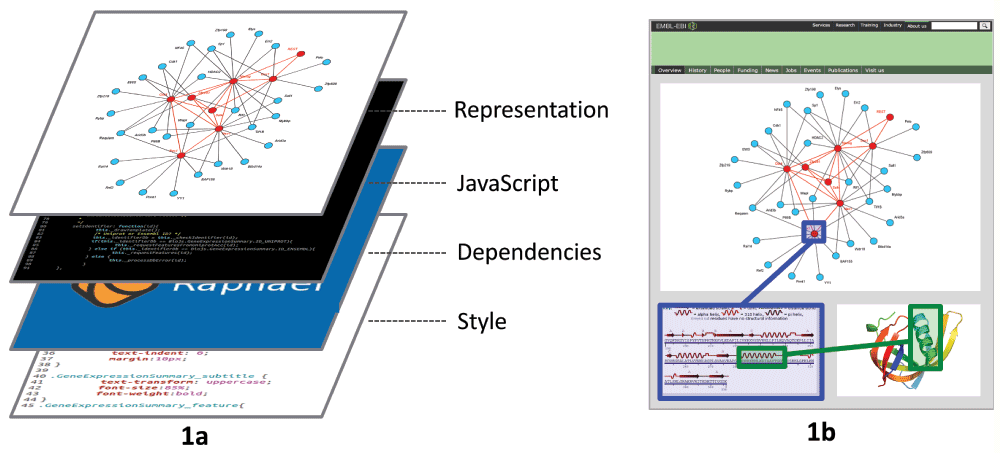
\includegraphics[width=\textwidth]{figures/biojs_layers.png}
\caption[BioJS layers.]{1a shows the different layers that a BioJS component is divided into. The representation layer sits on top of the JavaScript layer, which similarly possesses a layer of dependencies and a style. 1b presents an example of interactivity between three components, a protein-protein interaction network viewer, a secondary structure viewer and a tertiary structure viewer. 
\label{fig:biojs_layers}}
\end{figure}
 
The layer separation in the BioJS architecture is shown in the left side of figure \ref{fig:biojs_layers}. The final representation of a component can be deployed in any of the different methods supported in web, the control of such representation is programmed in JavaScript, supported by any of the libraries the developer choose to have as dependencies. If the chosen representation is based on HTML standards, all its elements can be stylised via Cascade Style Sheets CSS \cite{COR2014}.

Here are some examples of different methods to represent data in web with examples of BioJS components using them.
\begin{description}
\setlength\itemsep{-0.3em}
\item[HTML documents] Where HTML is generated to display data, for instance \emph{Biojs.InteractionsTable} (\url{http://www.ebi.ac.uk/Tools/biojs/registry/Biojs.InteractionsTable.html}) creates a HTML table that contains information about protein interactions (Figure \ref{fig:biojs_components} a).
\item[Visualizations using HTML elements] Similar to the previous one, but the HTML generated is organise in certain way to represent the data. For example,  \emph{Biojs.Chromosome} (\url{http://www.ebi.ac.uk/Tools/biojs/registry/Biojs.Chromosome.html}) uses the div HTML element to create boxes representing the bands of a chromosome (Figure \ref{fig:biojs_components} b).
\item[Scalable Vector Graphics] HTML supports the SVG format, and because SVG is a Markup language, its manipulation is similar to when dealing with HTML content. The \emph{Biojs.FeatureViewer} (\url{http://www.ebi.ac.uk/Tools/biojs/registry/Biojs.FeatureViewer.html}) uses this technique to display protein annotations (Figure \ref{fig:biojs_components} c).
\item[HTML canvas] Since HTML5 the element canvas is part of the specification, this component provides a programatic way to generate graphics. It is faster than SVG, but doesn't offer as much control on each of the drawn elements. For example, a representation of the metabolic pathways provided by KEGG is displayed by the \emph{Biojs.KEGGViewer} (\url{http://www.ebi.ac.uk/Tools/biojs/registry/Biojs.KEGGViewer.html}) component using the canvas element (Figure \ref{fig:biojs_components} d).
\item[Browser plugins] The use of third party tools such as Java Applets or Adobe Flash objects is also possible as long an interface with JavaScript is provided, for example \emph{Biojs.Protein3D} (\url{http://www.ebi.ac.uk/Tools/biojs/registry/Biojs.Protein3D.html}) displays the 3D structure of a proteins by using the JMol Java applet (Figure \ref{fig:biojs_components} e).
\end{description}

Besides the diversity in the chosen technology to represent the data, figure \ref{fig:biojs_components} also shows the variety of visualisation techniques that can be implemented using BioJS, from text tables to 3D objects.

\begin{figure}  
\centering
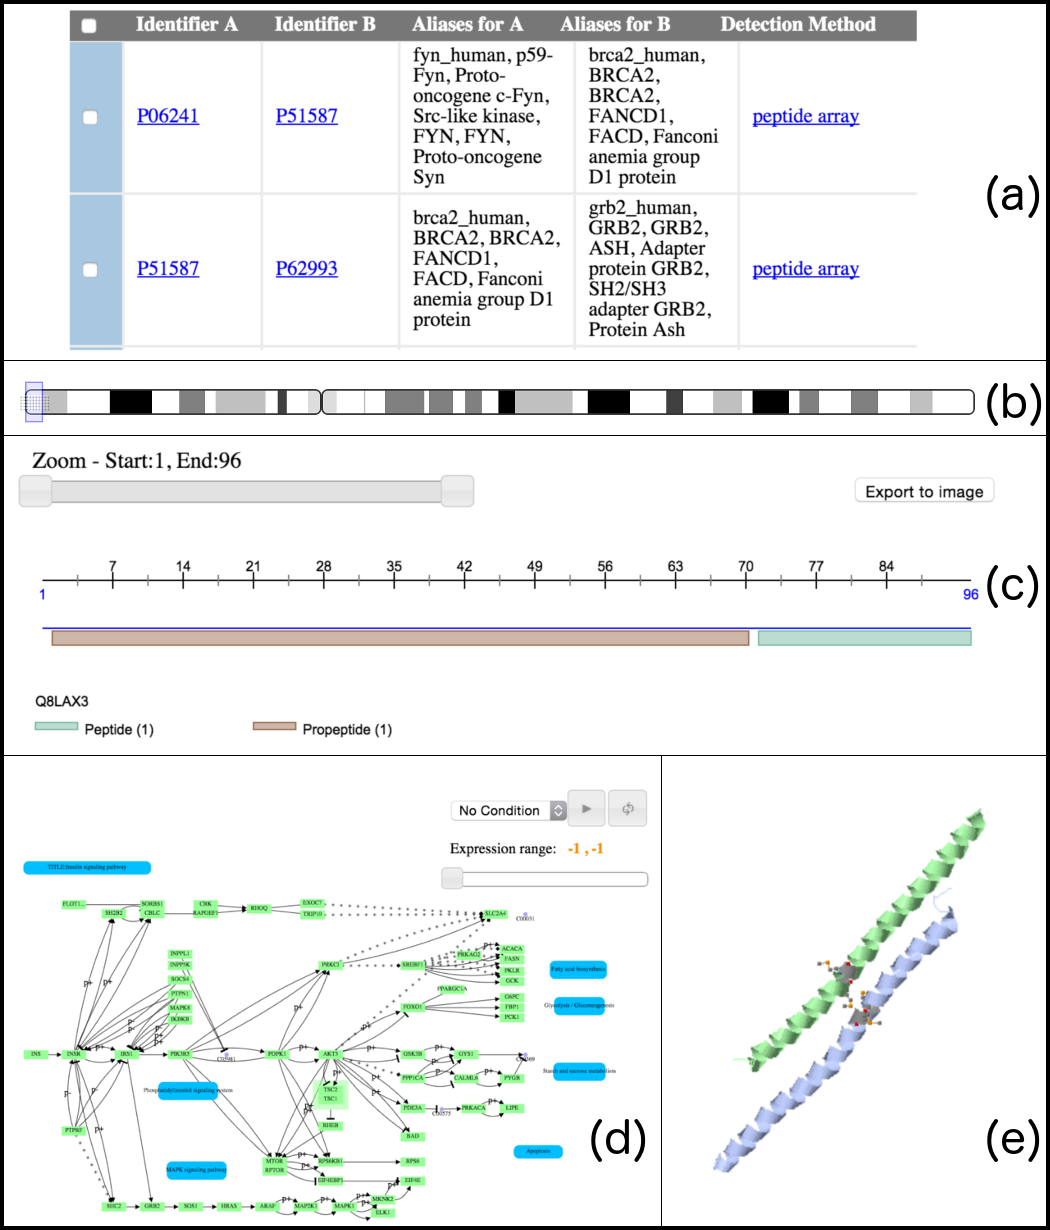
\includegraphics[width=\textwidth]{figures/biojs_components.png}
\caption[Snapshots of some BioJS components.]{Snapshots of some BioJS components. (a) Biojs.InteractionsTable, (b) Biojs.Chromosome, (c) Biojs.FeatureViewer, (d) Biojs.KEGGViewer and  (e) Biojs.Protein3D.
\label{fig:biojs_components}}
\end{figure}
 


BioJS ambitious vision is ``\emph{that every online biological dataset in the world should be visualised with BioJS tools}''. In order to accomplish it, BioJS requires to provide a convenient environment for the different roles related to the visualisation of biological data. The roles that we have identified are: data providers,  developers of web components, developers using ready-to-use components and the users that finally visit web tools that include those components.

A data provider can benefit from BioJS by simply reusing existing components that can visualise their type of data, and in this way save the resources that a development form scratch requires. Even if there is not component that fully covers the needs of the institution, is likely that there is a component that provide a partial solution, and thanks that BioJS an open-source project, the institution can extend the existing component, improving its feature set, or create an alternative version of it tailoring to the needs of the institution. In the case where the required representation is so unique, that the institution requires to develop the component from scratch, they still get the benefit of ensuring that anyone else who will display their data, will count with a widget that visualise it exactly in the way they intended to do so. The two last cases ultimately reflect in growth over the BioJS library for the benefit of other BioJS actors.

Developers creating new visualisations with BioJS can get exposure and acknowledgements for their efforts. Their widgets will be now visible in an open forum, where a community of potential users and collaborators can both, benefit and contribute to the improvement of the widget. On the technical side, a developer following the BioJS guidelines is not limited by any dependency, and although the need of writing documentation and applying a code structure, implies more time on the creation of the resource, it also ensures the robustness of the components.

When a developer wants to include a component to display some type of biological data, they can take advantage of BioJS by easily follow the common installation instructions provided in the registry, which have been customised for each of the components. The registry supports navigation and search of components, but we consider the bigger benefit for developers is to be able to run live demos of the components and the code to generate them. In this way, someone interested in a widget can seen it in action, without having to install or develop anything.

All of it has as the final beneficiary the researcher, who ultimately is the one who will interact with the different components getting a dynamic view of the data in the way the provider expected, in a component that can be improved by a community of visualisation experts, and has been chosen to be in the web tool that the user is visiting because it is the one that highlights the features of the data in the best way.

We are aware that this is still a work in progress, but the results so far obtained from the project are very positive. For example, the journal F1000research decided to publish an special collection of articles describing BioJS component. We have discussed before our opinion about how positive is for projects to provide an environment for the publication of peer-reviwed articles (Section \ref{subsubsec:ppi_biojs}). We consider that this collection of BioJS articles is an important step in the right path for the growth of the project and its contributions to the research community. The section \ref{subsubsec:ppi_biojs} describes the details of an article included in this collection, in which BioJS components for the visualisation of PPI networks are introduced.

\subsection{BioJS 2.0}
Besides the relative success of the first version of BioJS, its community identified a number of deficiencies and areas where the project can be improved. For example after BioJS first version was released, the focus of the community was directed to new components, and for around 3 years the core did not change much. During that time some of the libraries and strategies used got outdated, for example, the registry required compilation using maven (\url{http://maven.apache.org/}) in order to generate the web content for each of the components. This seemed a good idea at the beginning of the project, however became a problem because of the delay in the publication of components, and more importantly the lack of a protocol to retrieve the dependencies of each components.

The registry was still bringing visibility to the components, but it was failing to attract developers to create new widgets using the proposed guidelines. This was the main motivation to work on BioJS 2.0.

A concentrated effort looking to push forward the new version of BioJS was held during the 4th and 6th of August of 2014. The event was hosted in Munich Germany (\url{http://biojs.net/code/2014/07/04/announcing-hackathon.html}) and it was also possible to collaborate remotely. 

The motto of this event was to bring ``easiness'' back to BioJS. This principle has transcend from the event to become the goal of BioJS 2.0.  The efforts were mainly made from the point of view of the developer of new components: BioJS should be easy to develop, maintain and test, which should be done without failing to offer the benefits to the other BioJS stake holders and therefore BioJS should continue to be easy to use, combine and discover.

The main strategy to be able to provide the desired ``easiness'' was to give freedom to the developer, which in BioJS terms meant to deprecate the predefined class where all the components used to inherit, it also implied to abolish the requirement to follow the JSDoc format to document and introduce easily editable, working examples of an component and moving the documentation to a public README file or any other form chosen by the developer (e.g. github wiki).

The alternative was to define a set of guidelines called ``the gold standard" (\url{http://edu.biojs.net/series/102/70_gold_standard.html}). It includes recommendations on how to test, document, publish and create examples for a BioJS component. The key behind these recommendations is that all of them are supported by web resources that can be accessed programatically. The registry is then able to detect when a recommendation is followed by a component, and present this information to users exploring the components. For example, the sniper package (\url{https://github.com/biojs/sniper}) facilitates the inclusion of live examples in the component's page.

This implementation in the registry was done by extensively use two well know development resources available in the web: The web-based Git repository hosting service: GitHub; and the node package manager (npm). 

All the code of BioJS was migrated to the source control system git (\url{http://git-scm.com/}) and the repositories are hosted by GitHub (\url{https://github.com/biojs/}). The source code of the components is now independently manage by their authors, and the only components in the BioJS repository are the ones related with the core functions, such as the registry or helpers to follow the gold standard.

A developer creating a BioJS component should publish its code as a npm package (\url{https://www.npmjs.com/}). npm is in itself a registry of packages for javascript components, which has programmatic access from a command line client, but also can be browsed using its online front end (\url{https://www.npmjs.com}). All the configuration and metadata of a npm package should be included in a file named package.json, which should be located at root of the package folder. BioJS builds upon this standards and added custom fields for meta information to the package.json file.

%One of the reasons why npm has been chosen as a base technology for BioJS is the way it manages the dependencies of a package: when a npm package is installed all its dependencies are automatically downloaded, including recursive ones (i.e. when a dependency has dependencies). In this way BioJS 2.0 solves what was a big issue of its previous version. 

By February 2015 npm had more than 120000 packages in its repository, with an extraordinary growth rate of 221 packages per day, as reported by the independent website \url{http://www.modulecounts.com/}. The high adoption of the npm repository is an advantage for BioJS developers because it provides an extensive tool set to work with, which scope goes beyond the visualisation of biological data.

With this model, the developer is now free to use any package to accomplish any of the BioJS guidelines, and as long it is reported in the package.json file it can be reported in the BioJS registry. The reporting of the gold standard implemented features it is still a work in progress, nonetheless a fully operational registry for BioJS2.0 is available at \url{http://biojs.io/}.

It is important to highlight the continuous effort from the BIoJS community to provide up to date documentation . The web portal \url{http://edu.biojs.net/} contains tutorials and reference documents to help the developers of new BioJS components.

\begin{figure}  
\centering
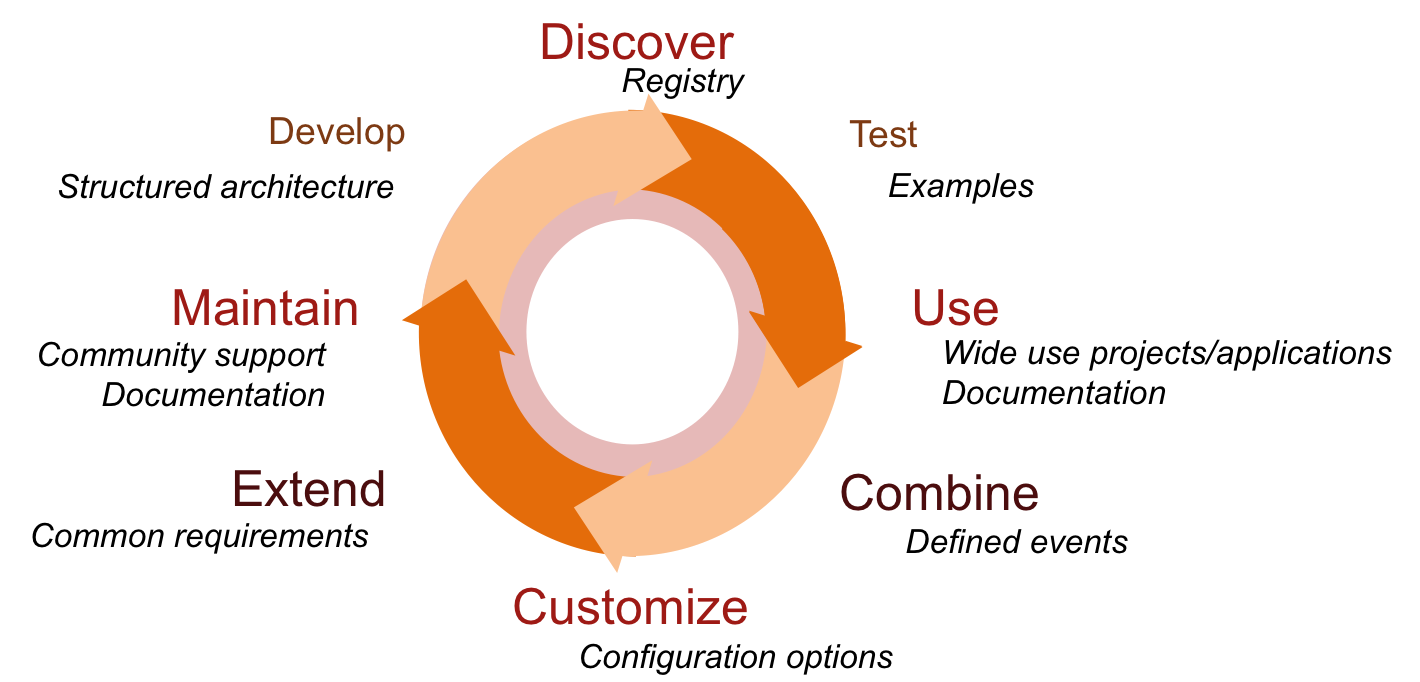
\includegraphics[width=\textwidth]{figures/biojs_cycle.png}
\caption[Cycle of a BioJS component]{Cycle of a BioJS component.
\label{fig:biojs_cycle}}
\end{figure}

Figure \ref{fig:biojs_cycle} represents the development stages of  a BioJS component, below we describe some of the technical details on how BioJS 2.0 assists in each of these stages.

\subsubsection{Develop}
The developer is free to use any javascript framework or visualisation library as a dependency. the only requirement is to report them in the package.json file. Ideally the dependencies should also be npm packages, in order to support recursive checking. However is also possible to include required files as part of the package. 

There is an assistant package to generate a template for a BioJS project (\url{http://biojs.io/d/slush-biojs}). The package was created using Slush(\url{https://slushjs.github.io}) and once executed, it includes some dependencies and configurations useful to comply some of the guidelines in the BioJS gold standard.

\subsubsection{Discover}
The only requirement for a npm package to be included in the BioJS 2.0 repository is to contain the tag ``\emph{biojs}'' in the package.json file. The BioJS registry queries npm to check for published packages with the ``\emph{biojs}'' tag and processes their configuration files in order to extract all the information about documentation, tests, etc.% and to dynamically generate with it, the content that other users will find about this component.

%The registry displays all the npm packages that are tagged with ``\emph{biojs}'' and t
The developer is free to use other tags in order to better describe its component. Anyone interested in a visualisation component for biological data, can visit \url{http://biojs.io/} and then search by keywords, check what are the most popular components or the most recently updated. Each component page contains the documentation that the developer has included.

\subsubsection{Test}
Users interested in a component can try it out in the same registry page, if an snippet of the code was reported by the developer. The registry also provides links to execute the examples through online javascript editors such as JS Bin (\url{http://jsbin.com/}) or codepen (\url{http://codepen.io/}), which allow the user to edit the sample code to edit parameters and basically to have a playground area to test out the component.

On the developer side, the use of npm supports the execution of unit tests through several frameworks such as mocha (\url{http://mochajs.org/}), qunit (\url{http://qunitjs.com/}) or jasmine (\url{http://jasmine.github.io/}). All of which are available in the npm repository; thanks to this, all the unit tests can be ran by the execution of a a single npm command. 

Freely available web resources such as travis(\url{https://travis-ci.org/}) or drone.io (\url{https://drone.io/}) can be setup to automatically run the tests every time new code is pushed to the github repository of the component. If provided, this information can be used by the BioJS registry when creating the component's page. In this way, explorers of biological components will know if the latest version of the code have passed all the unit tests.

\subsubsection{Use}
The simplest way to use a BioJS 2.0 component is to install it through the npm command line tool:
\begin{lstlisting}[language=csh]
npm install <package_name>
\end{lstlisting}

To be able to run this command, the npm tool needs to be installed and it should have internet access. If this is the case, the components will be downloaded together with all its dependencies and extras included in the package (e.g. snippets and docs). 

The developer can include other commands in the configuration of the file that can be executed once installed, for example to run tests, generate documentation, built minified versions of the code, etc.

It is also possible to configure a compiled version of the component that includes all the dependencies in a single file and serve it using a Content Delivery Network (CDN), which then provides a way to use the component on any web page by only including a single line in the header of the HTML. The author of a BioJS component can use the npm package browserify-cdn, which is a convenient way to publish via CDN.

\subsubsection{Combine}
Several BioJS components can be included in the same web page and displaying them simultaneously. However this method does not allow interactivity between the components, and to accomplish that, some programming in Javascript is required.
 
As describe before npm provides support to handle dependencies, therefore to combine BioJS components, it is possible to write another npm package that declares the desired components as dependencies. Moreover, thanks to some tools such as CommonJS (\url{http://www.commonjs.org/}), Browserify (\url{http://browserify.org/}) and RequireJS (\url{http://requirejs.org/}) it is possible to declare when a component is required using JavaScript code. This provides a way to built a unified javascript that contains all the components and the code to integrate them.

The dynamic interaction between components can be reached through the broadcasting of events from one component, and the reaction to it form another one. As mentioned before, BioJS 2.0 removed the parent class where the uniform event handler was implemented, however a recommended BioJS component called biojs-events (\url{http://biojs.io/d/biojs-events}) is now provided to supply this need.

\subsubsection{Customize}
Each BioJS component defines the parameters need it to run an instance of it. The input of such parameters can be defined in several ways, for example, as attributes of the constructor of a JavaScript object, or as a configuration file, or even as HTML parameter on the element where the component will be included.

This mean that the level of customisation and the methods to do it are responsibility of the developer of the component. However we consider that is common understanding from BioJS developers that the ability of personalise a component it is an important feature and its documentation should be included as part of the package.

\subsubsection{Extend}
Since BioJS 2.0 there is not common repository for all the components, this decision, delegates the responsibility to manage the code that is been published through the repository to the developers. And it also allows the use of source control repositories such as GitHub, in which any developer can obtain the source code of the component, extend it and request the changes to be included in a future version.

This strategy gives the control of contributions, and extensions to the owner of the component, while liberating the members of the BioJS team from tasks related to that administration of particular components.

Alternative a developer can always copy an open source component, what in GitHub terminology is known as ``\emph{fork a repo}'', extend it to implement new features, or to use it with a different purpose of the original developer, and then create another BioJS component from it.

\subsubsection{Maintain}
The maintenance of a component is again responsibility of its author in BioJS 2.0. By supporting this process with GitHub the developer can take advantage of the multiple tools provided by this service. For example, \emph{branching} to experiment with the code without affecting the current release, or to have a list of \emph{issues} where users can report bugs or suggestions, or even receive improvements from other users directly in the code via a \emph{pull request}.

The BioJS registry includes the latest version of the code published in npm. Versioning is a fundamental part of npm, it uses the standard known as SemVer (\url{http://semver.org/}) to specify if changes are: \emph{patches}, where bugs or changes that don't alter the functionality of the package are done; (ii) \emph{minor} releases that include new features that are backwards compatible; or  \emph{major} releases, when the new features have incompatibilities with previous versions.

Every time a package is publish in npm it requires a new version number. In this way users of a package can specify which version to install in order to ensure the correct behaviour of their components.

\subsection{Developed Components} \label{subsec:biojs_components}
Besides the contributions in the development and maintenance of BioJS we have created a few BioJS components that are currently listed in the registry. The components described below were originally developed for BioJS 1.0, but have been updated to version 2.0. This process was manually implemented in the case of the Chromosome Viewer, in order to explore and test the new features of the registry. In contrast, the upgrading of the PPI components, mentioned at the end of this section, was achieved with a tool developed to upgrade all the components from the first version into BioJS 2.0.

An article that is part of the BioJS series in the F1000 research journal describes the components for the display of PPI networks using a force directed layaout and a circle layout. The first author of the publication is Gustavo A. Salazar and the co-authors provided input in their role of collaborators and supervisors.

\subsubsection{Chromosome Viewer}
We designed and developed a BioJS component to display a chromosome that includes the reported cytogenetic bands. The original version of this component is available in the BioJS 1.0 registry (\url{http://www.ebi.ac.uk/Tools/biojs/registry/Biojs.Chromosome.html}) and there is also an updated version for  BioJS 2.0 (\url{http://biojs.io/d/biojs-vis-chromosome}).

Cytogenetic bands are the result of an experimental technique that dyes chromosomes in such a way that regions with higher percentage of the nucleotides adenine and thiamine are dark, while guanine and cytosine rich areas are light. This colour code is usually a good indication of areas with less (dark) or more (light) genes. The exposure of this bands help in the identification of chromosomes, and it is also useful to easily localise a genomic region in a chromosome.

The naming convention for the bands in a chromosome divides the bands in two groups physically marked by the position of the centromere, which is the region where a chromosome links with its pair. This division creates a short and a long arm, which are marked as p and q respectively. The bands are then numbered starting from the centromere as p1, p2, etc. for the short arm, and q1, q2, etc, for the long one; and more numbers can be used to name sub regions that are detected in higher resolution \cite{NLM2013}.

\begin{figure}[ht]
\centering
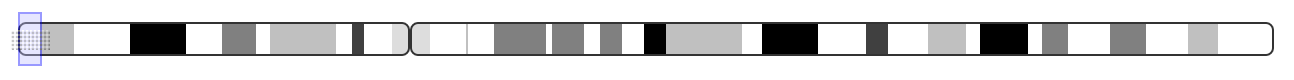
\includegraphics[width=\textwidth]{figures/chromosome.png}
\caption[BioJS component to represent a Chromosome]{BioJS component to represent a Chromosome
\label{fig:biojs_chromosome}}
\end{figure}

Figure \ref{fig:biojs_chromosome} is an snapshot of the BioJS component displaying chromosome 8 from \emph{Homo sapiens}. The information is obtained from the DAS server provided by Ensembl that contains the karyotype information (\url{http://www.ensembl.org/das/Homo_sapiens.NCBI36.karyotype/features?segment=8}). The DAS response is processed using JsDAS, extracting information about the chromosomic location, name and category of each band, which ultimately defines where, what label and which colour will be used to paint the region in the component.

The chromosome is represented in a web page by a composition of HTML div elements, where all the divs are drawn on the same line without any separation between themselves. CSS classes are defined for each of the chromosome categories, for example the style below will be assign to the div that is rendered with a gpos25  category.

\begin{lstlisting}[language=HTML]
.gpos25 {
	background-color: rgb(25%, 25%, 25%);
}
\end{lstlisting}

The border of the bands at both edges of the chromosome and the ones next to the centromere are rounded in order to visually identify these areas (as seen in figure \ref{fig:biojs_chromosome}).

The component broadcast events when the user hovers or clicks over a band, in the examples this is used to display a label or to reposition an area selector over the corresponding bar. This area selector is an utility BioJS component (\url{http://www.ebi.ac.uk/Tools/biojs/registry/Biojs.AreaSelector.html}), that although is not biological related, it can be reused by any component that uses a similar approach to the graphic representation (i.e. HTML elements). Figure \ref{fig:biojs_chromosome} shows the selector over the band that is at the left of the chromosome. The selected region can be manipulated by dragging the edges of the blue area, and every time a new area is marked, events are broadcasted and other BioJS component can react accordingly.

In BioJS 2.0 is recommended to only publish biological related components, therefore we decided to exclude the Area selector component from the BioJS registry. Nonetheless the component was published in npm (\url{https://www.npmjs.com/package/area_selector}) and can be reused by other npm packages including those part of BIoJS
 
\subsubsection{Protein-Protein Interactions Force Layout} \label{subsubsec:ppi_biojs}
The most popular way to visualise networks is known as the node-link metaphor, in which some figures (e.g. circles. squares, images) represent the nodes; and lines connecting them are the links. When the network consists of a short amount of nodes, it is possible to specify the position for all of them, however when the amount of nodes grows, the effort required to position all of them also increases and random location of nodes would probably generates highly congested graphics with overlapping of elements and very cluttered areas.

Different strategies have been defined to automatically organise network representations. We have used the implementation of a force-directed layout included in the D3 library (\url{https://github.com/mbostock/d3/wiki/Force-Layout}) \cite{BOS2011} for the BioJS component that can visualise protein-protein interaction networks in a web native component:  \url{http://www.ebi.ac.uk/Tools/biojs/registry/Biojs.InteractionsD3.html}, \url{http://biojs.io/d/biojs-vis-interactions-d3}.

The force directed layout implemented in D3 follows the simile of attaching springs to all the connected nodes, in this way  two nodes connected pull towards each other, and if a node has several links it is subjected to all the spring forces of its connections at the same time. The algorithm also includes a rejection force between all the nodes, which aims to disperse unconnected nodes and avoid cluttered areas. An optional gravity point can be setup where all the nodes are attracted, this helps to keep the nodes in the visible area. 

The simulation of the movement of the nodes caused by the defined forces is executed by steps. For each step, all the forces affecting a node are used to calculate a new position for it, and this is done for all the nodes. An internal temperature parameter is used to control the speed of change during each step: when the simulation starts the temperature is high and the particles move fast, and with each iteration the network gets closer to an stable position dropping the temperature, and the nodes move slower as a consequence. The use of the temperature parameter also helps to stop completely the simulation when is lower than a predefined value, this with the purpose of avoiding unnecessary CPU use.The simulation might be required to restart when for example new nodes or links are added to the network, in which case the temperature parameter is changed to a high value.

In order to optimise the number of operations required on each step, the D3 implementation includes a data structure called quadtree that creates a hierarchical organisation of the nodes based in their location. This is used when calculating the rejection forces of each node, so instead of considering all the rejection forces, an aggregated value for the nodes in a region can be used.

A quadtree divides the area in quadrants, the root of the tree contains all the nodes and it has four branches. The first branch contains the nodes that are located in the first quadrant of the graphic (i.e. between the top-left corner and the centre of the graphic), the second branch includes the nodes inside the second quadrant, etc. The same division can be recursively calculated for each quadrant.

The decision on how deep in the structure the algorithm should go to calculate the rejection forces is based on the criterium known as Barnes-Hut \cite{BAR1986}. If the quotient between the width of the quadrant \emph{s} and the distance from the node to the centre of the quadrant \emph{d} is less than a threshold value $\theta$, the aggregated force of the quadrant is sufficient and the recursion on the tree can be stopped. 
%The equation is manipulated to avoid the use of square roots and is written into the D3 library as the conditional:

%\begin{lstlisting}[language=java]
%if (dw * dw / theta2 < dn) 
%\end{lstlisting}

An step in the simulation is concluded when all the forces of all the nodes have been use to calculate the new positions of all the nodes. And every time an step concludes, an event called \emph{tick} is broadcasted. Listeners of the event, can then alter the behaviour of the simulation by adding other forces, for instance to contain the nodes in a frame, or to define several gravity points. The event is also useful to trigger changes in the graphic representing the network, and in this way to animate the simulation.

For the BioJS PPI force layout component we used the \emph{tick} event not only to display the simulation but also to  define multiples \emph{foci} of gravity, one for each organism reported as a protein, in this way the proteins that belong the same organism get attracted to the same area.

The representation of the network in the browser has been implemented using SVG. Path elements forming symbols are used to represent proteins of different organisms. We took advantage of the SVG technology by allowing the user to freely zoom and pan around the graphic with popular mouse gestures i.e. scrolling for zooming and dragging for panning, owever, if the user is dragging the mouse over one of the figures representing a protein, only that node gets moved and once the mouse id released, the protein is forced to stay in the position were the user drops it, this action restarts the simulation in  order to find positions for the rest of the proteins in the graphic.

A running example of this component has been published in \url{http://jsfiddle.net/Bvh6k/8/} using JSFiddle (\url{http://jsfiddle.net/}), an online resource that supports the edition and live execution of snippets of Javascript code. Details on the biological entities used in the example can be found in \cite{SAL2014}. Figure \ref{fig:biojs_force} is an snapshot of the visualisation generated by this example. 

\begin{figure}[ht]
\centering
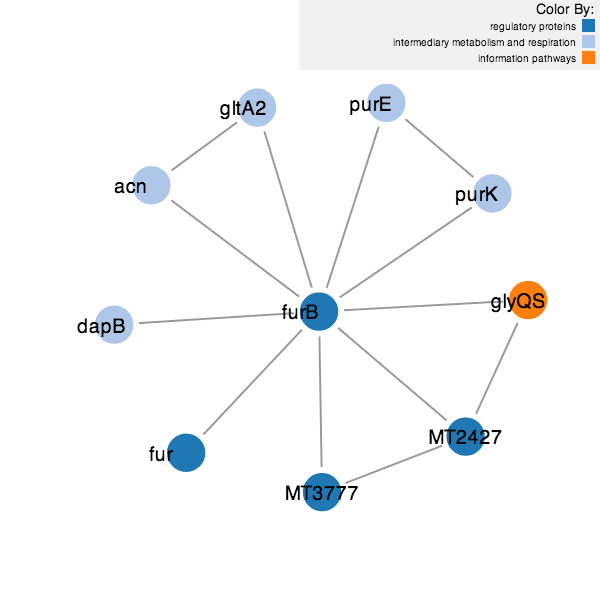
\includegraphics[width=5in]{figures/force.png}
\caption[BioJS component to represent a network using the force-directed layout]{BioJS component to represent a network using the force-directed layout
\label{fig:biojs_force}}
\end{figure}

Besides allowing developers to experiment with the code, the example serve us to explain the use of the component. 

A developer should start by creating an instance of the component:

\begin{lstlisting}[language=java]
var instance = new Biojs.InteractionsD3({
   target: "example"
});
\end{lstlisting}
					
All the proteins in the graphic should then be added. The following example shows how to add the protein with UniProt id O05839 (\url{http://www.uniprot.org/uniprot/O05839}). Note how the organism to which it belongs is included, along with which feature should be used for the label:

\begin{lstlisting}[language=java]
instance.addProtein({
      id: "O05839", organism: "MTB",
      gene_name:"furB",
      typeLegend:"gene_name"});
\end{lstlisting}
					
In the same way, the interactions should be added to the graphic, making sure that the interactions are between proteins that have already been added. For instance:

\begin{lstlisting}[language=java]
instance.addInteraction(
      "O05839", "P0A582",
      {id: "P0A582_P0A582"}); 
\end{lstlisting}
					
Once all the proteins and interactions have been declared, the graphic can be restarted so it reflects the additions:

\begin{lstlisting}[language=java]
instance.restart ();
\end{lstlisting}

The example also includes some instructions for colouring and format. 


\subsubsection{Protein-Protein Interactions Circle Layout} \label{subsubsec:ppi2_biojs}
We have developed another component to display PPI networks that uses the D3 implementation of a circle layout: \url{http://www.ebi.ac.uk/Tools/biojs/registry/Biojs.InteractionsBundleD3.html}. In this layout the proteins are organised in a circle, positioning all the nodes around the centre without favouring any of them, this can help to discover connection patterns around the network (Figure \ref{fig:biojs_circle}). 

The interactions in this visualisation are spline curves which path is defined through the hierarchical edge bundle algorithm \cite{HOL2006}. This algorithm requires the data to be organised in a hierarchy, and in the case of been used in combination of a circle layout, the non-leave nodes of the tree are organised following a radial pattern, where the root of the tree is in the centre, and first level children are located in a circumference around it, the nodes of the following level of the tree are position in a circumference of bigger radius around the root. The same is then done for all the levels of the hierarchy. The nodes in the last level, which are the leaves of the tree, are the only visible ones.

When an interaction between two nodes is drawn, the curve's path will be created using the hierarchy nodes as guidelines. This method highlights the links between two highly connected groups in the hierarchy, because all of those connections will follow a similar inner path, creating the impression of a bundled connection, hence the name of the algorithm.

The hierarchy used for the BioJS component to display PPI network is a two level tree, that simply separates the proteins by organism, which is useful when looking to multi-organism networks such as a host-pathogen scenario. Another case of multi-organisms is discussed in section \ref{sec:orthologs}, where pseudo-interactions were defined to identify a relationship between two orthologs.

\begin{figure}[ht]
\centering
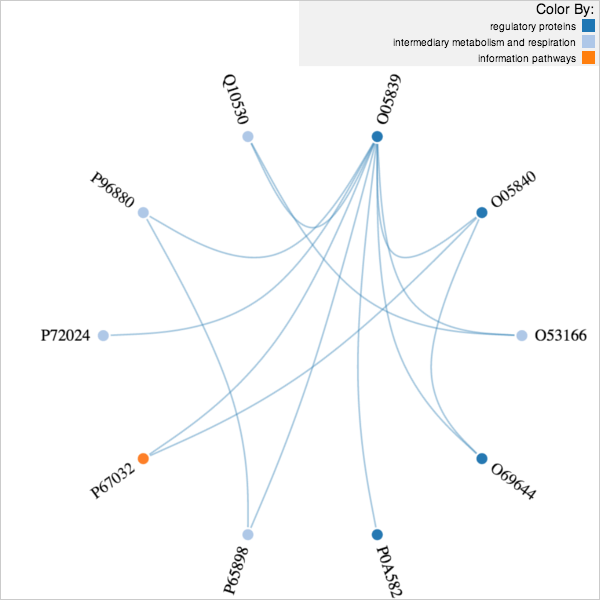
\includegraphics[width=5in]{figures/circle.png}
\caption[BioJS component to represent a network using the circle layout]{BioJS component to represent a network using the circle layout
\label{fig:biojs_circle}}
\end{figure}

Figure \ref{fig:biojs_circle} shows an snapshot of the component displaying the same dataset as the example for the force-layout component, which has been also uploaded as a JsFiddle: \url{http://jsfiddle.net/J4CE7/9/}.

Both components follow the same API (Application Program Interface) and therefore any script developed to display on one layout can be used on the other. The only difference between the APIs is because of methods that help to control the force layout of the first component which do not apply to the Circle layout. Thanks to this, the script to generate a PPI visualization of the same network is very similar in both.  The only difference between the two scripts loaded in JsFiddle is the declaration of the object. Instead of using the object Biojs.InteractionsD3 it uses Biojs.InteractionsBundleD3 and rest of the script is exactly the same.
\begin{lstlisting}[language=java]
var instance = new Biojs.InteractionsBundleD3({
    target: "example",
});
\end{lstlisting}





\subsubsection{Protein-Protein Interactions Heat Map} \label{subsubsec:ppi3_biojs}
After the publication of \cite{SAL2014} where we described the two components explained in the previous sections, we decided to explore an alternative to visualise PPI interactions. A new BioJS component was developed to visualise the interactions as a matrix of proteins by proteins, similar to the way that some heat maps are used in the processing of microarrays or phylogenetics analysis, but in this case not all the squares of the matrix are filled, only those marking an interaction between two proteins are painted. The component is now in the BioJS 2.0 registry (\url{http://biojs.io/d/biojs-vis-interactions-heatmap-d3}) and the source code is freely available in GitHub (\url{https://github.com/4ndr01d3/biojs-vis-interactions-heatmap-d3}).

This method to visualise PPI networks put the emphasis of the graphic in the interactions rather than in the proteins. And by sorting the matrix and using a correct colouring of the protein labels, for instance based in the functional class, it is possible to find features that other wise aren't evident in a node-link representation because the overlapping of the interaction lines.

Figure \ref{fig:biojs_heatmap} is a snapshot of this component  in which random interactions of 15 fake proteins are displayed. We have included extra functionality in the example to demonstrate the use of some of the methods and events provided in the API of the component. The mouse pointer in the figure is located over the cell that remarks the interaction between \emph{prot\_2} and \emph{prot\_15}, hence the lines crossing over it. We have also clicked on that interaction cell, which triggers an event that displays two panels with the feature information of the interacting proteins. The size of panels and graphic have been optimised for better use the available space on the SVG container.

The interactions in the example have been coloured using a scale between red and green based in the other this proteins are included into the model. This feature can be used to represent any quantifiable value associated with the interaction, for example evidence scores.

\begin{figure}[ht]
\centering
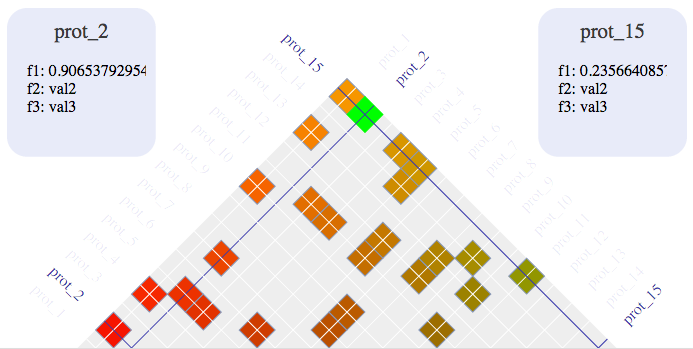
\includegraphics[width=\textwidth]{figures/heatmap.png}
\caption[BioJS component to represent a network using a heat map]{BioJS component to represent a network using a heat map
\label{fig:biojs_heatmap}}
\end{figure}

An interactive example of this component can be accessed directly form the BioJS registry (\url{http://workmen.biojs.net/jsbin/biojs-vis-interactions-heatmap-d3/simple_example}). In this case we are using a different tool called JSBin, which behaves similarly to JsFiddle, the tool used in the examples of the previous components. JSBin has a better support for the inclusion of npm packages and therefore it is easier to use with BioJS 2.0 components.

The component also shares the same API as the previous two PPI visualisation widgets, which makes it easy to alternate the view between the 3 PPI components and in this way offer to the user several options to display their data.


\subsection{Discussion}
We have discussed in the introduction (section \ref{sec:ppi}) the existence of several tools that visualise PPI networks; all of which support variations of a force-directed layout. However by the time we developed the components described in this section, there were not web components to create such visualisations using HTML5 web standards. We are aware now of the existence of the Cytoscape.js project, which offers an alternative based in the HTML5 element canvas and include implementations of not only force-directed layouts but also circle, grid, and others. Nonetheless, we consider that is important to have technology alternatives  for this type of components. If for example, a developer is already using D3 in its web tool, the use of our components can be a better alternative to reduce the network latency created by many dependencies.


\section{PINV, a web-based Protein Interaction Network Visualiser }  \label{section:pinv}
Protein-protein interaction data has been used in multiple research scenarios: (i) to browse networks for genes of interest, (ii) to interpret the results of genome-wide genomic screen, (iii) to interpret functional genomics data and (iv) to elucidate disease genes \cite{FRA2013}. In all of them visualisation has play an important role, where is to for instance,  to meaningful navigate around a big network (i and iv), to find clusters of proteins with shared functionalities(iii and iv)  or highlight links that are not evident with other techniques (i and ii).

The web is a platform for cooperative efforts, where the roles for authors and readers, providers and consumers; are harder to distinguish.

\subsection{Architecture}
json config file
widgets

\subsection{Implementation}
\subsection{Description of the application}
%\subsection{Use Cases}

\subsection{Spacial clustering for big networks on a force-directed layout}

\section{Discussion}


